\documentclass[11pt,a4paper]{article}

% ---------------------------------------------------------------------------
% Packages
% ---------------------------------------------------------------------------
\usepackage[margin=2.3cm]{geometry}
\usepackage[T1]{fontenc}
\usepackage{lmodern}
\usepackage{microtype}
\usepackage{graphicx}
\usepackage{booktabs}
\usepackage{tabularx}
\usepackage{array}
\usepackage{amsmath}
\usepackage{enumitem}
\usepackage[table]{xcolor}
\usepackage{caption}
\usepackage[section]{placeins}
\usepackage[numbers,sort&compress]{natbib}
\usepackage[colorlinks=true,linkcolor=blue!50!black,citecolor=blue!50!black,urlcolor=blue!50!black]{hyperref}

\graphicspath{{figures/}}
\setlist{itemsep=2pt,topsep=4pt}
\setlength{\emergencystretch}{1.5em}
% Stack floats at the top of float-only pages instead of spreading them out
\makeatletter
\setlength{\@fptop}{0pt}
\setlength{\@fpsep}{14pt plus 4pt}
\setlength{\@fpbot}{0pt plus 1fil}
\makeatother
\renewcommand{\topfraction}{0.85}
\renewcommand{\bottomfraction}{0.6}
\renewcommand{\textfraction}{0.1}
\renewcommand{\floatpagefraction}{0.75}
\setcounter{topnumber}{3}
\setcounter{totalnumber}{5}
\captionsetup{font=small,labelfont=bf}
\renewcommand{\arraystretch}{1.15}
\newcolumntype{L}{>{\raggedright\arraybackslash}X}

% Feature names in typewriter font (escape underscores as \_)
\newcommand{\feat}[1]{\texttt{#1}}

% Highlighted placeholder for unfinished parts. Delete before submission.
\newcommand{\todo}[1]{\par\smallskip\noindent\fcolorbox{orange}{yellow!15}{%
  \parbox{\dimexpr\linewidth-2\fboxsep-2\fboxrule\relax}{\small\textbf{To do:} #1}}\par\smallskip}

% ---------------------------------------------------------------------------
\title{Sampling Sensitivity of Global SHAP Feature Rankings in\\Short-Term Electricity Demand Forecasting}
\author{David Kelly \qquad Xuanwei Xu\\[6pt]
  \small FIT2082 Computer Science Research Project 13\\
  \small Monash University\\[2pt]
  \small Supervisor: Zeehan Saleheen}
\date{}

\begin{document}
\maketitle


% ===========================================================================
\begin{abstract}
Global SHAP feature rankings are widely used to explain machine-learning load forecasts, yet they depend on two sampling choices that are rarely examined: the background sample and the set of predictions explained. This study measured how these choices affect the stability and reliability of rankings for a LightGBM model forecasting Victorian electricity demand 24 hours ahead. Three background methods, four background sizes, five evaluation methods and two evaluation sizes were crossed and each configuration was repeated with 30 random seeds, giving 3{,}600 exact TreeSHAP runs. Whole rankings were highly repeatable under every design (Kendall's $W$ 0.963--0.997), but the top five features were not: explaining holidays and temperature extremes changed the top five in 27.6\% of runs, against 1--2\% for ordinary sampling, as daily maximum temperature rose towards fifth place. SHAP rankings agreed substantially but not completely with permutation importance (mean Spearman correlation about 0.83), and removal-and-retraining confirmed that calendar and temperature features carry predictive value; the larger cost of removing temperature on rare-event days was suggestive but not statistically established. A 50-row background with 500 evaluation rows matched the largest configuration's top-five stability at about a quarter of the cost; the top ten needed 100 rows, and rare-event explanations kept improving up to the largest size tested, making 100 rows plus averaging across seeds the practical choice. Rankings should be reported with their sampling design, and separately for rare conditions where those conditions matter.
\end{abstract}

% ===========================================================================
\section{Introduction}

Accurate short-term electricity demand forecasting underpins power-system operation, energy scheduling and the balance between supply and demand~\cite{pinheiro2023}. Machine-learning models capture the complex relationships between demand, weather, calendar effects and past consumption, but their complexity makes it hard for analysts and operators to see how a forecast was produced. Interpretability therefore matters alongside accuracy, especially when forecasts support operational decisions~\cite{baur2024}.

SHapley Additive exPlanations (SHAP) assign each input feature a contribution to an individual prediction~\cite{lundberg2017}. Averaging the absolute contributions across many predictions gives a global feature-importance ranking, which load-forecasting studies have used to identify the relative importance of historical demand, weather and calendar features and to guide feature selection~\cite{lee2023,vanzyl2024}.

These rankings depend on two choices that are usually treated as technical details. The \emph{background sample} defines the reference against which contributions are measured, and the \emph{evaluation sample} determines which predictions are explained and averaged. Different sizes, random draws or selection strategies can therefore yield different rankings. Earlier work found that SHAP values and rankings fluctuate across random backgrounds, with the instability shrinking as the background grows~\cite{yuan2023}, and that deliberately biased background sampling can change SHAP explanations substantially~\cite{laberge2023}.

The problem is sharper in electricity demand forecasting, where some features matter greatly under specific conditions yet appear unimportant when averaged over ordinary periods. Public holidays and extreme weather are rare but can change demand substantially. Van Zyl et al.\ showed that SHAP rankings could support feature selection in energy forecasting, but also that SHAP could underestimate infrequent yet important features and produce rankings not fully supported by feature-ablation experiments~\cite{vanzyl2024}.

An explanation existing does not make it trustworthy: explanations that change under small, reasonable variations give a misleading account of a model~\cite{alvarezmelis2018}. This report distinguishes two properties:
\begin{itemize}
  \item \textbf{Stability:} repeating the SHAP analysis with different samples produces similar global rankings.
  \item \textbf{Reliability:} features ranked highly genuinely contribute more to forecast accuracy than those ranked low.
\end{itemize}

Existing studies have examined background sample size outside the energy domain~\cite{yuan2023}, applied SHAP rankings to load forecasting without testing their stability~\cite{lee2023,vanzyl2024}, or compared rankings between normal and extreme-weather regimes as a secondary analysis~\cite{abubakkar2026}. To our knowledge, how background and evaluation sampling \emph{jointly} affect both the stability and the reliability of global SHAP rankings in electricity demand forecasting has not been systematically studied.

\subsection{Aim and research questions}

This project aims to determine how the selection of background and evaluation samples affects the stability and reliability of global SHAP rankings in short-term electricity demand forecasting, and to produce evidence-based, computationally efficient sampling recommendations for practitioners. Three research questions build on one another towards this aim:

\begin{description}[leftmargin=1.2cm,style=nextline]
  \item[RQ1] How do the size and construction method of background and evaluation samples jointly affect the stability of global SHAP feature rankings in short-term electricity demand forecasting?
  \item[RQ2] Do SHAP rankings generated under different sampling conditions reliably reflect features' genuine predictive contribution, as assessed through feature-ablation experiments and agreement with permutation feature importance?
  \item[RQ3] What is the smallest background and evaluation sample configuration that produces rankings comparable in stability and reliability to those generated using the largest available samples?
\end{description}

RQ1 establishes whether rankings are stable and what drives instability. Stability alone is not enough, since a design could consistently rank the wrong features, so RQ2 tests whether rankings are also correct. RQ3 combines both to identify the cheapest configuration that is stable and reliable, turning the findings into practical guidance (Table~\ref{tab:rq-map}).

\begin{table}[htbp]
\centering\small
\caption{Where each research question is addressed.}
\label{tab:rq-map}
\begin{tabular}{lll}
\toprule
Question & Methods & Results \\
\midrule
RQ1 & Sampling design and stability metrics (\S\ref{sec:design}, \S\ref{sec:metrics}) & \S\ref{sec:rq1} \\
RQ2 & Reliability checks (\S\ref{sec:reliability}) & \S\ref{sec:rq2} \\
RQ3 & Paired size comparisons and cost (\S\ref{sec:metrics}) & \S\ref{sec:rq3} \\
\bottomrule
\end{tabular}
\end{table}

\subsection{Contributions}
\begin{itemize}
  \item A systematic study of how background and evaluation sampling jointly affect the stability of global SHAP rankings in electricity demand forecasting: 120 configurations, each repeated with 30 seeds, extending prior work that examined background size alone~\cite{yuan2023}.
  \item An evaluation of rare-event-stratified explanation, testing whether holidays and extreme temperatures change the ranking of infrequent but high-impact features, as Van Zyl et al.\ suggested~\cite{vanzyl2024}.
  \item A combined stability-and-reliability framework, using ablation and permutation importance to check whether reproducible rankings also reflect genuine predictive contribution.
  \item Practical recommendations on the sample sizes needed for stable and reliable rankings at reduced computational cost.
\end{itemize}

Section~\ref{sec:background} reviews related work, Section~\ref{sec:methods} describes the methods, Section~\ref{sec:results} presents results for each research question, and Section~\ref{sec:discussion} discusses their implications and limitations.

% ===========================================================================
\section{Background and related work}\label{sec:background}

This section reviews four bodies of work: load forecasting and its growing use of explanation, how SHAP computes explanations for tree models, evidence that SHAP is sensitive to sample selection, and how explanations can be validated. It closes with the gap this project addresses.

\subsection{Load forecasting and the need for explanation}

Short-term load forecasting supports operational decisions across power systems~\cite{pinheiro2023}. Weather and calendar effects, particularly temperature, day of week and public holidays, are consistently identified as dominant drivers of short-term load~\cite{hong2016}, and combining demand data with weather and calendar covariates is standard practice in explainable load forecasting~\cite{machlev2022}. These findings justify this project's feature set.

Reviews of explainable AI in load forecasting~\cite{baur2024} and in energy and power systems more broadly~\cite{machlev2022} describe its rapidly growing use. As explanations increasingly inform how forecasts are trusted and used, whether those explanations are themselves dependable becomes a practical question, not only an academic one.

\subsection{SHAP and explanations for tree models}

SHAP attributes a prediction to its input features using Shapley values from cooperative game theory, unifying several earlier additive attribution methods~\cite{lundberg2017}. For an arbitrary model, Shapley values must be approximated by sampling. For tree ensembles, TreeSHAP computes them exactly in polynomial time, and aggregating its local explanations produces global importance rankings~\cite{lundberg2020}.

This distinction is central to the design here. Pairing an exact method with a gradient-boosted tree model, LightGBM~\cite{ke2017}, means any variation between rankings cannot come from approximation error in the explanation algorithm, so it can be attributed to sampling. By contrast, sampling-based SHAP estimators carry their own estimation uncertainty~\cite{slack2021}, and drawing background rows can also create input combinations that never occur in real data, which recent load-forecasting work avoids with sampling-free SHAP variants~\cite{hertel2026}. In TreeSHAP's interventional mode, contributions are measured relative to a background sample, which is often compressed with $k$-means into a smaller representative set~\cite{lundberg2017}. Which background is used changes what the explanation means: Chen et al.\ showed that explaining the same prediction against different reference groups shifts which features appear important, and recommended clustering-based backgrounds for this reason~\cite{chen2022}. Both the size and the construction of the background are therefore treated as experimental variables.

\subsection{Sensitivity of SHAP to sample selection}

Several studies show that SHAP output depends on the data used to compute it. Yuan et al.\ found that SHAP values and feature rankings vary across randomly sampled backgrounds, with variation decreasing as background size increases; they also observed that the most and least important variables were ranked more reliably than moderately important ones~\cite{yuan2023}. Liu et al.\ showed, in clinical prediction, that the balance and composition of both background and explanation data affect SHAP explanations~\cite{liu2022}. Laberge et al.\ went further, showing that a background sample chosen with deliberate bias can sharply reduce a feature's apparent importance while remaining statistically hard to detect~\cite{laberge2023}.

Together these suggest that both the background and the evaluation sample matter. However, none of these studies concerns energy forecasting, none jointly varied the size, composition and construction method of both samples under repeated sampling, and none tested whether the resulting rankings reflect genuine predictive importance. This project addresses all three. A further, theoretical result sharpens the concern: Bhattacharjee et al.\ proved that a small mean $|\text{SHAP}|$ over the data does not by itself show that a feature is irrelevant, and that whether it does depends on the distribution the values are averaged over~\cite{bhattacharjee2025}. The evaluation sample is exactly that distribution.

Instability can also come from the model rather than the samples. Yasodhara et al.\ found that SHAP rankings for tree ensembles degrade under model perturbation and noisy features~\cite{yasodhara2021}, and Caraker et al.\ showed that, with correlated features, gradient boosting concentrates importance on whichever feature it happens to split on first, so rankings change between training seeds~\cite{caraker2026}. This project holds one frozen model fixed so that the sampling effect can be isolated.

\subsection{Validating explanations}

Alvarez-Melis and Jaakkola argue that robustness, meaning similar explanations under similar conditions, is a prerequisite for trusting an interpretability method~\cite{alvarezmelis2018}. This motivates the stability measurement in RQ1.

Stability, however, does not show that a ranking is correct. Permutation importance, which measures how much forecast error rises when a feature's values are shuffled, offers an independent check: it is model-agnostic, does not use Shapley values, and has been applied to feature selection in load forecasting~\cite{huang2016}. Combined with feature ablation, it provides the reliability test in RQ2. The two properties can genuinely diverge: in fraud detection, Bhuiyan et al.\ found SHAP rankings that were stable across dataset variants yet agreed only weakly with permutation importance~\cite{bhuiyan2026}. Explanation methods more generally often disagree about which features matter, which Krishna et al.\ quantify with top-$k$ and rank-agreement measures similar to those used here~\cite{krishna2022}.

\subsection{SHAP rankings in load forecasting}

Lee et al.\ applied SHAP-based feature importance to short-term load forecasting and used it for feature selection, but did not test whether the rankings stay stable under repeated sampling~\cite{lee2023}. Van Zyl et al.\ compared SHAP with Grad-CAM for feature selection in national energy-demand forecasting~\cite{vanzyl2024}. They found that SHAP could underestimate infrequent but important features, and that its rankings were not fully supported by feature-ablation experiments. That finding is the most direct motivation for this project: it suggests that how the explained predictions are chosen may decide whether rare conditions register at all, which motivates rare-event-stratified evaluation in RQ1 and ablation in RQ2.

Hao et al.\ measured SHAP ranking stability in cross-building load forecasting, using Spearman correlation and top-10 overlap across cross-validation folds and between seen and unseen buildings, and found the rankings largely consistent~\cite{hao2026}. Their comparison changes the data and model folds together, so it does not isolate the SHAP sampling choices studied here.

Most recently, Abubakkar et al.\ computed SHAP rankings separately for normal and extreme-weather periods in ERCOT load forecasting, finding that temperature rose to the top rank during extreme events, and checked ranking stability over 20 bootstrapped backgrounds~\cite{abubakkar2026}. Their study shows that regime-specific rankings differ, but treats this as part of an interpretability framework for one deep-learning model rather than as a controlled study of sampling choices, and does not test whether the regime-specific rankings are reliable.

\subsection{Research gap}

Table~\ref{tab:gap} summarises how the closest studies relate to this project.

\begin{table}[htbp]
\centering\small
\caption{Closest related studies and how this project differs.}
\label{tab:gap}
\begin{tabularx}{\linewidth}{>{\raggedright\arraybackslash}p{2.3cm} >{\raggedright\arraybackslash}p{2.9cm} L L}
\toprule
Study & Domain and model & Focus & Difference from this project \\
\midrule
Liu et al.~\cite{liu2022} & Clinical prediction, deep learning & Balance and composition of background and explanation data & Outside energy; no systematic comparison across sample sizes; no reliability validation \\
Yuan et al.~\cite{yuan2023} & Clinical (ICU), deep learning & Background size and SHAP stability & Varies background size only; this project jointly varies both samples' size and construction method \\
Laberge et al.~\cite{laberge2023} & Fairness auditing, tree and neural models & Adversarially biased background sampling & Studies deliberate manipulation, not the effect of ordinary design choices \\
Hao et al.~\cite{hao2026} & Cross-building load forecasting & Ranking stability across folds and buildings & Varies data and model together; SHAP samples not varied \\
Lee et al.~\cite{lee2023} & Short-term load forecasting & SHAP importance for feature selection & Same domain; ranking stability not tested \\
Van Zyl et al.~\cite{vanzyl2024} & Energy-demand forecasting, CNN & SHAP vs.\ Grad-CAM, with feature removal & Evaluates usefulness of rankings; does not isolate sampling effects \\
Abubakkar et al.~\cite{abubakkar2026} & ERCOT load, CNN--Transformer ensemble & Normal vs.\ extreme-event SHAP rankings & One background design; regime comparison secondary; reliability not tested \\
\textbf{This project} & Short-term demand, LightGBM with exact TreeSHAP & Stability and reliability of global rankings & Varies both samples systematically, repeats every configuration 30 times, validates with ablation and permutation importance \\
\bottomrule
\end{tabularx}
\end{table}

% ===========================================================================
\section{Methods}\label{sec:methods}

The study holds one accurate forecasting model fixed and varies only how SHAP samples are drawn, so any change in the resulting feature rankings can be attributed to sampling. The work proceeded in five stages:
\begin{enumerate}
  \item Build a five-minute electricity demand dataset with weather and calendar features.
  \item Train, tune and freeze a LightGBM forecaster, validated against a seasonal-naive baseline.
  \item Explain the frozen model with TreeSHAP under 120 sampling configurations, each repeated with 30 seeds (RQ1, RQ3).
  \item Measure ranking stability within and between configurations, and test which factors affect it.
  \item Check whether stable rankings reflect genuine predictive importance (RQ2).
\end{enumerate}

\subsection{Data and forecasting model}\label{sec:data}

The target is Victorian (VIC1) operational demand at five-minute resolution from 1 January 2024 to 31 December 2025, retrieved from AEMO's dispatch data~\cite{aemo2025} with the NEMOSIS package~\cite{gorman2018}. It was combined with three supporting sources (Table~\ref{tab:sources}).

\begin{table}[htbp]
\centering\small
\caption{Supporting data sources.}
\label{tab:sources}
\begin{tabularx}{\linewidth}{L L l}
\toprule
Source & Content & Resolution \\
\midrule
Bureau of Meteorology, Melbourne (Olympic Park), station 086338~\cite{bom2025} & Daily minimum and maximum temperature & Daily \\
Renewables.ninja (MERRA-2)~\cite{pfenninger2016,staffell2016}, \url{www.renewables.ninja} & Solar irradiance, simulated PV output, modelled temperature & Hourly \\
Victorian public holiday calendar & Holiday flag; day of week, weekend and season derived from timestamps & Daily \\
\bottomrule
\end{tabularx}
\end{table}

Daily and hourly values were assigned to every five-minute interval they cover. The resulting 26 model features fall into four groups: demand history (11 lags and rolling statistics), weather (7), time of day and year (5), and calendar flags (3).

The forecasting task is day-ahead: from each forecast origin, predict demand 24 hours (288 intervals) later. This horizon is standard in short-term load forecasting and reflects operational scheduling. Weather features are taken from the forecast origin rather than from the target time 24 hours later, which a real forecaster could not observe. One qualification applies: each daily temperature value covers a whole day (the BOM daily maximum spans 9~am to 9~am the next morning), so origins early in a day see temperatures that occur later that day. Section~\ref{sec:limitations} discusses the implications.

The data was split chronologically into training (70\%), validation (15\%) and test (15\%) sets, with a 288-interval gap between consecutive sets. The gap equals the forecast horizon, so no training target falls inside the validation period and no validation target inside the test period (Table~\ref{tab:splits}).

\begin{table}[htbp]
\centering\small
\caption{Chronological splits.}
\label{tab:splits}
\begin{tabular}{lrl}
\toprule
Split & Rows & Forecast origins \\
\midrule
Training & 143{,}723 & 15 Jan 2024 -- 28 May 2025 \\
Validation & 30{,}797 & 29 May 2025 -- 13 Sep 2025 \\
Test & 30{,}799 & 14 Sep 2025 -- 29 Dec 2025 \\
\bottomrule
\end{tabular}
\end{table}

LightGBM~\cite{ke2017} was chosen because gradient-boosted trees perform well on tabular load-forecasting data and, crucially, support exact TreeSHAP computation~\cite{lundberg2020}. An exact method removes explanation-algorithm approximation as a source of variation, so any instability observed comes from sampling. The model used an L1 (mean absolute error) objective. Three candidate hyperparameter settings were compared on validation MAE with early stopping, and the test set was used only once, after selection. The selected model (learning rate 0.03, 63 leaves, 678 boosting rounds, seed 2082) achieved the accuracy in Table~\ref{tab:accuracy}.

\begin{table}[htbp]
\centering\small
\caption{Forecast accuracy of the frozen model against the seasonal-naive baseline.}
\label{tab:accuracy}
\begin{tabular}{lrrr}
\toprule
Split & LightGBM MAE (MW) & Seasonal-naive MAE (MW) & Improvement \\
\midrule
Validation & 367.91 & 491.40 & 25.1\% \\
Test & 397.49 & 524.05 & 24.1\% \\
\bottomrule
\end{tabular}
\end{table}

The seasonal-naive baseline predicts that demand 24 hours ahead equals current demand. Clearly beating it was a precondition: explanations of an inaccurate model would say little about the system it models. Once approved, the model, feature set, split boundaries and exact input file were frozen for all later experiments.

\subsection{SHAP explanation and verification}\label{sec:shap}

Each run explains the frozen model with TreeSHAP in interventional mode~\cite{lundberg2020}. A row's SHAP value for a feature measures how much that feature moves the prediction away from the average prediction over a background sample. The global ranking for a run is the mean absolute SHAP value of each feature across the rows of an evaluation sample.

Interventional mode was required because it is the only TreeSHAP mode that uses the background sample; the alternative, tree-path-dependent mode, relies on statistics stored in the trees and ignores the background entirely. Varying the background would then have no effect, making RQ1 untestable.

Two safeguards ensured the explainer did what the design intended:
\begin{itemize}
  \item \textbf{Background size is enforced explicitly.} By default, the SHAP library silently subsamples any background larger than 100 rows. The background was therefore passed through an explicit masker with its full size, without which the 200-row backgrounds would have been truncated without warning.
  \item \textbf{Every run is checked for additivity.} SHAP values must satisfy $\text{prediction} = \text{base value} + \sum \text{SHAP values}$ for each row. Each run records its largest reconstruction error, warns above $\max(5\,\text{MW}, 1\%)$ of the median prediction and stops above $\max(5\,\text{MW}, 5\%)$, a level that a genuine wiring error, such as misaligned features, would exceed by orders of magnitude.
\end{itemize}

Most rows reconstructed to within 0.001~MW, but a few showed gaps of up to about 110~MW. A diagnostic run traced these to feature values lying exactly on a tree split threshold, where LightGBM and SHAP's internal copy of the tree route the row down different branches. For the worst row, increasing \feat{temperature} (10.9) by one part in a million changed the model's prediction by 109.55~MW, exactly matching that row's error. Such ties are frequent here because daily and hourly weather values are repeated across every five-minute interval they cover.

An earlier explanation, that the gaps came from the L1 objective, was rejected after a plain L1 model reconstructed exactly when tested in isolation. The effect on rankings is bounded: a run's ranking totals can shift by at most the summed row errors divided by the evaluation size, 1.15~MW in the diagnosed run against gaps of tens of MW between features. Across all 3{,}600 runs, 1{,}068 raised a warning and none reached the hard limit.

\subsection{Sampling design}\label{sec:design}

Five factors were fully crossed, giving 120 configurations ($3 \times 4 \times 5 \times 2$), each run with 30 seeds for 3{,}600 runs in total (Table~\ref{tab:design}).

\begin{table}[htbp]
\centering\small
\caption{Experimental factors and the reason for each.}
\label{tab:design}
\begin{tabularx}{\linewidth}{>{\raggedright\arraybackslash}p{2.6cm} >{\raggedright\arraybackslash}p{4.4cm} L}
\toprule
Factor & Levels & Why \\
\midrule
Background method & Uniform; $k$-means; time-stratified & Uniform is the neutral baseline; $k$-means is the standard way to summarise a SHAP background~\cite{lundberg2017}; time-stratified guarantees coverage of the year and the day \\
Background size & 25, 50, 100, 200 rows & Spans cheap to costly settings, to locate where stability stops improving (RQ3) \\
Evaluation method & Uniform; time-stratified; season-stratified; rare-event-stratified; outcome-demand-stratified & Tests whether \emph{which} predictions are explained changes the ranking, including the rare conditions SHAP is suspected to underweight \\
Evaluation size & 100, 500 rows & Tests whether averaging over more predictions stabilises the ranking \\
Seed & 30 per configuration (2082--2111) & Yields a distribution of rankings per configuration rather than a single draw \\
\bottomrule
\end{tabularx}
\end{table}

Background samples were drawn only from the training split, representing the data the model learned from. Evaluation samples were drawn only from the test split, representing unseen predictions. The two pools never overlap, so no row serves as both reference point and explained prediction. Each run's evaluation sample used seed $+\,100{,}000$, keeping background and evaluation draws independent.

The construction methods work as follows:
\begin{itemize}
  \item \textbf{Uniform:} simple random sampling.
  \item \textbf{$k$-means:} the features are standardised, clustered into as many clusters as the background size, and the real row nearest each cluster centre is kept. Real rows are used rather than synthetic centres so every background row is a genuine observation. Missing values (two incomplete weather days) are median-filled for the clustering step only; the rows returned are unchanged.
  \item \textbf{Time-stratified:} proportional allocation across calendar month and four six-hour blocks of the day, up to 48 strata.
  \item \textbf{Season-stratified:} proportional allocation across the four seasons. Because the test split spans 14 September to 29 December, only spring and early summer are present.
  \item \textbf{Rare-event-stratified:} half the sample from rare rows and half from ordinary rows. A row is rare if it falls on a public holiday or its daily mean temperature lies outside the training split's 5th--95th percentile range (9.45--26.35\,\textdegree C). Rare rows are a small minority, so drawing them in proportion would differ little from uniform sampling; deliberate over-sampling tests whether emphasising them changes the ranking.
  \item \textbf{Outcome-demand-stratified:} half the sample from rows whose realised demand 24 hours later exceeded the training 95th percentile (6{,}780~MW). Because this uses the future outcome, it is treated as a retrospective cohort, kept separate from rare-event sampling, which selects on conditions of the forecast day rather than on the demand being forecast.
\end{itemize}

All thresholds were fixed from the training split before any SHAP run, so ``rare'' and ``high demand'' mean the same thing in every run and cannot be tuned to the results.

\subsection{Stability metrics and statistical analysis}\label{sec:metrics}

Stability was measured at two levels, because repeating a design and changing a design answer different questions.
\begin{itemize}
  \item \textbf{Within-condition stability} asks whether repeating the same sampling design gives the same ranking. For each configuration, all 435 pairs of its 30 seeds were compared, and agreement across all 30 seeds was summarised with Kendall's $W$.
  \item \textbf{Between-condition agreement} asks whether changing the design changes the answer. Each configuration's consensus ranking (mean $|\text{SHAP}|$ per feature over its 30 seeds) was compared with the consensus of a reference configuration: a uniform 200-row background with a uniform 500-row evaluation sample, the largest setting, following the proposal's use of the largest sample as the stable reference. The \emph{reference top five} are the five features with the highest mean $|\text{SHAP}|$ in that configuration, averaged over its 30 seeds: \feat{lag\_5min}, \feat{day\_of\_week}, \feat{day\_of\_year}, \feat{origin\_hour\_of\_day} and \feat{lag\_10min}. The reference is used in two ways. Each single run's top five is compared with it, to measure how often one run gives a different answer; and each configuration's consensus top five is compared with it, to test whether averaging over seeds recovers the same answer.
\end{itemize}

Four metrics were used, because they capture different aspects of agreement (Table~\ref{tab:metrics}).

\begin{table}[htbp]
\centering\small
\caption{Stability metrics.}
\label{tab:metrics}
\begin{tabularx}{\linewidth}{>{\raggedright\arraybackslash}p{3.2cm} L L}
\toprule
Metric & What it compares & How to read it \\
\midrule
Spearman $\rho$ & Positions of all 26 features in two rankings & 1 = identical order, $-1$ = reversed \\
Kendall $\tau$ & Every pair of features: same relative order in both rankings? & Stricter than Spearman, since every swapped pair counts \\
Kendall's $W$ & Agreement across all 30 seeds of a configuration at once & 0 = no agreement, 1 = identical \\
Top-$k$ Jaccard ($k=5,10$) & Which features are in the top $k$, ignoring order: shared $\div$ distinct & 1 = same set; 0.43 = only 3 of the top 5 shared \\
\bottomrule
\end{tabularx}
\end{table}

Whole-ranking metrics are dominated by the many lower-ranked features, whose order rarely changes, so they can mask changes at the top, where feature-importance decisions are made. Top-$k$ Jaccard isolates the top, following the top-$k$ agreement measures used to compare explanations~\cite{krishna2022} and SHAP rankings in load forecasting~\cite{hao2026}. Kendall's $W$ used average ranks with the standard tie correction, since features with zero importance tie exactly.

Statistical tests used configuration-level values (one per configuration), because seed pairs within a configuration are not independent:
\begin{itemize}
  \item \textbf{Factor effects (RQ1):} a Kruskal--Wallis test for each factor and metric, followed by Dunn's pairwise tests. Each test pools over the other factors; because the design is fully crossed, every level sees each combination of the other factors equally often. Holm correction was applied across all tests.
  \item \textbf{Smallest sufficient size (RQ3):} each configuration was paired with the configuration identical in every respect except size, and the two compared with a Wilcoxon signed-rank test (30 pairs per background size, 60 for evaluation size), Holm-corrected. Since a non-significant difference does not prove equivalence, the median difference is reported alongside every $p$-value. The trend in stability with background size was summarised by regressing each metric on $\log_2$ of the size.

  A configuration was defined as \emph{sufficient} for a given metric when two conditions held: (i)~its paired difference from the largest configuration was not statistically detectable (Holm-adjusted Wilcoxon $p \ge 0.05$), and (ii)~doubling its background size improved the mean of that metric by less than 0.01. For top-five Jaccard, a gain of 0.01 means roughly one pair of runs in thirty agreeing on one more feature, which was judged negligible against the roughly doubled computation time that a doubled background costs. The 0.01 threshold is a judgement rather than a standard value, so the results report the underlying numbers alongside the recommendation. Because rare-event evaluation behaved differently, sufficiency was assessed separately for it; with only six matched pairs per size, condition~(i) could not be tested there, so condition~(ii) was applied alone.
  \item \textbf{Uncertainty in importance:} 95\% bootstrap confidence intervals on each feature's mean $|\text{SHAP}|$ within a configuration, from 2{,}000 resamples of its 30 seeds.
\end{itemize}

\subsection{Reliability checks (RQ2)}\label{sec:reliability}

A stable ranking is not necessarily a correct one: a sampling design could consistently rank the wrong features highly. RQ2 therefore checks rankings against two measures that do not use Shapley values: permutation importance of the frozen model, and feature ablation with retraining. They measure different things, and neither is a ground truth. Both use the same 24-hour-ahead task, 26 features and chronological splits as the SHAP experiment; the test set contains 30{,}799 forecast origins.

\subsubsection{Permutation importance and comparison with SHAP}
Permutation importance is the increase in test MAE when a feature's values are shuffled, without retraining the model~\cite{huang2016}. Negative values, where shuffling slightly improved accuracy, were kept rather than set to zero. On the full test set, each of the 26 features and each of the six feature groups in Table~\ref{tab:rq2groups} was shuffled ten times. Within a group, all columns were shuffled together, so their relationships with each other were preserved. The spread across the ten repeats reflects shuffling variability only, not a confidence interval.

\begin{table}[htbp]
\centering\small
\caption{Feature groups used in RQ2. Counts sum to the frozen model's 26 features.}
\label{tab:rq2groups}
\begin{tabularx}{\linewidth}{l r L}
\toprule
Group & Count & Features \\
\midrule
Temperature & 4 & \feat{temp\_min}, \feat{temp\_max}, \feat{temperature}, \feat{irr\_temperature} \\
Irradiance & 3 & \feat{irr\_electricity}, \feat{irr\_irradiance\_direct}, \feat{irr\_irradiance\_diffuse} \\
Recent demand & 3 & \feat{lag\_5min}, \feat{lag\_10min}, \feat{lag\_15min} \\
Seasonal demand & 4 & \feat{lag\_1day}, \feat{lag\_1week}, \feat{demand\_lag\_288}, \feat{demand\_lag\_2016} \\
Rolling demand & 4 & \feat{roll\_mean\_1h}, \feat{roll\_std\_1h}, \feat{roll\_mean\_24h}, \feat{roll\_std\_24h} \\
Calendar & 8 & \feat{day\_of\_week}, \feat{is\_weekend}, \feat{is\_public\_holiday}, \feat{origin\_hour\_of\_day}, \feat{hour}, \feat{minute}, \feat{month}, \feat{day\_of\_year} \\
\bottomrule
\end{tabularx}
\end{table}

To compare with the SHAP grid, the 300 evaluation samples (five methods, two sizes, 30 seeds) were reconstructed with the shared sampler, using each saved grid seed plus the evaluation-seed offset of 100{,}000. Each feature in each sample was shuffled once, giving 7{,}800 measurements. Thus, the 30-seed variability combines evaluation-sample selection and donor-permutation randomness; it is not 30 shuffles of one fixed sample. Signed MAE increases were averaged across the 30 seeds before ranking and compared with the matching 30-seed mean absolute SHAP ranking using Spearman correlation, Kendall's $\tau$ and top-5 and top-10 Jaccard, giving 120 configuration comparisons. Configurations with the same evaluation method and size share one permutation ranking across all background methods and sizes, so these comparisons are not independent replications or formal tests of background design.

The supplied SHAP archive did not store evaluation row identifiers or model/data content hashes. Reconstructed feature order, split boundaries, sample coverage and frozen-model baseline metrics were checked, but those compatibility checks cannot independently establish that the reconstructed samples contain exactly the original SHAP rows.

\subsubsection{Rare-event days and feature ablation}
Rare-event days use the same definition as rare-event sampling (Section~\ref{sec:design}): a public holiday, or a daily mean temperature at or below 9.45~$^\circ$C or at or above 26.35~$^\circ$C, the training split's 5th and 95th percentiles. The test set contains 2{,}016 rare-event rows on seven dates and 28{,}783 ordinary rows on 100 dates. Membership is fixed from unmodified forecast-origin data, not target demand or shuffled temperatures. As a supplementary check, temperature values were also shuffled only within the same cohort (rare or ordinary), to see how much the permutation result depends on where the shuffled values come from.

Ablation removed each feature group in turn, and separately removed \feat{temp\_max} alone, then retrained on the original training split only. The two exact duplicate seasonal-lag pairs were removed together within the seasonal-demand group. Each reduced model was compared with a full-feature model trained with the same seed, at seeds 2082, 2083 and 2084: eight variants (one full model and seven removals) at three seeds, giving 24 fits. Hyperparameters and the 678 boosting rounds were kept fixed, with no retuning or early stopping, and the frozen SHAP model was left unchanged. For a removed group $g$, seed $s$ and cohort $C$, the paired change is
\[
\Delta\mathrm{MAE}_{g,s,C}
=\mathrm{MAE}_{g,s,C}-\mathrm{MAE}_{\mathrm{full},s,C}.
\]
Reported MAE and RMSE changes are averaged over these three paired training seeds, not measured against the separately saved frozen baseline. Positive changes mean worse forecasts; negative changes are retained.

For each fitted pair, 2{,}000 bootstrap draws resampled the 107 whole forecast-origin dates with replacement, retaining paired reduced/control errors within each date. Rare and ordinary mean error changes were recomputed using the same date weights, and their difference was taken within each draw. The 2.5th and 97.5th percentiles give the reported 95\% interval. Draws without observations in a required cohort were omitted; 1{,}998 valid draws remained for each temperature rare-minus-ordinary contrast. This preserves within-day dependence, but does not account for longer-than-day dependence or uncertainty from drawing a new training set. Intervals are conditional on each fitted model pair, not pooled across the three training seeds. Only seven rare-event dates are available.

\paragraph{Limitations of these checks.}
The ablations remove feature groups rather than each configuration's own top five against its bottom five, as originally planned, so they cannot on their own confirm the smallest reliable configuration for RQ3. Correlated features, such as the several demand lags, can stand in for one another when one is removed, and shuffling can create unrealistic combinations of values. Because hyperparameters were fixed, removing columns also slightly changes the effective feature-subsampling rate. The temperature comparison was chosen after seeing the RQ1 results and reuses the same test period, so it is exploratory rather than a confirmation on fresh data. Finally, the daily-temperature look-ahead (Section~\ref{sec:limitations}) applies here as well.

\subsection{Implementation and reproducibility}\label{sec:implementation}

The pipeline was implemented in Python as separate modules for data acquisition, training, sampling, the experiment grid and analysis, version-controlled on GitHub, with major contributions reviewed through pull requests. After adding the RQ2 package, 87 automated tests passed across the repository and RQ2 suites. They cover the data merge, leakage guards in the training split, sampling methods, stability metrics, the experiment runner and RQ2 invariants and saved-table checks. For example, the Kendall's $W$ implementation is checked against its known identity with mean pairwise Spearman correlation.

Because the grid took several hours, the experiment runner was built to fail early and recover safely:
\begin{itemize}
  \item \textbf{Preflight:} one sample of every method and size is built before any SHAP run, so configuration errors surface in seconds. This caught a $k$-means failure on missing temperature values before the main run started.
  \item \textbf{Resume:} each run is saved as it completes, so an interrupted grid continues rather than restarts, and extra seeds or sizes compute only the new runs.
  \item \textbf{Manifest guard:} the runner refuses to add results to a folder produced from a different model or dataset.
\end{itemize}

Freezing the exact input file, not only the code, proved necessary. Early in the project, a model retrained from the same code, configuration and seed produced similar but different results (test MAE 402.84 against 397.49~MW). The cause was a different input file with 16 rather than 26 features, which a feature-list check exposed. From then on, the model and its exact input file were shared as a pair.

All SHAP runs used a laptop, without high-performance computing. Before extending the grid to more background sizes, a single seed of each new configuration was timed to estimate the full cost. SHAP computation averaged between 2.6 seconds per run (25-row background, 100-row evaluation) and 33.3 seconds (200 and 500 rows), about 10 hours in total. The grid-analysis script regenerates the RQ1/RQ3 stability tables and figures. The separate \texttt{rq2/} package supplies the permutation and ablation code, protocol, original result tables and a standard-library audit that rebuilds the RQ2 paired-error summaries, sample-size agreement tables and top-five membership comparisons without loading a model or rerunning experiments. Provenance records the original input/result hashes and distinguishes the packaged source from the historical run/audit snapshots; exact historical executable identity is not claimed.

\subsection{Departures from the proposal}\label{sec:departures}

The design was adjusted in six places, each for a practical or methodological reason (Table~\ref{tab:departures}).

\begin{table}[htbp]
\centering\small
\caption{Departures from the project proposal.}
\label{tab:departures}
\begin{tabularx}{\linewidth}{>{\raggedright\arraybackslash}p{2.6cm} >{\raggedright\arraybackslash}p{2.6cm} >{\raggedright\arraybackslash}p{3.1cm} L}
\toprule
Aspect & Proposal & Final & Reason \\
\midrule
Demand resolution & Half-hourly & Native five-minute & Supervisor direction: keeps AEMO's dispatch resolution without resampling \\
Weather features & Half-hourly temperature and humidity & Daily temperature (BOM) and hourly irradiance (Renewables.ninja) & Free BOM station data is daily and has no humidity; irradiance added on supervisor advice, since rooftop solar strongly shapes daytime demand \\
Hyperparameter tuning & Time-series cross-validation & Three candidates compared on one purged chronological validation split, with early stopping (50 rounds) & Keeps tuning chronological and leakage-free at lower cost; robustness across several time folds was not tested \\
Background sizes & 25, 50, 100, 250, 500 & 25, 50, 100, 200 & Compute cost; sizes added incrementally after timing, as advised by the supervisor \\
Evaluation sizes & 10\% to 100\% of the test set & 100 and 500 rows & SHAP cost grows with evaluation size; the full test set (30{,}799 rows) across 3{,}600 runs was impractical on a laptop \\
Evaluation methods & Random, season-stratified, rare-event-stratified & Added time-stratified and outcome-demand-stratified & Time-stratified mirrors the background method; outcome-demand isolates high-demand periods, kept separate because it uses future information \\
\bottomrule
\end{tabularx}
\end{table}

The smaller size ranges limit RQ3: stability could not be traced beyond a 200-row background or a 500-row evaluation sample, so the largest tested setting stands in for ``the largest available samples''.

% ===========================================================================
\section{Results}\label{sec:results}

All results come from 3{,}600 SHAP runs: 120 sampling configurations, each repeated with 30 seeds, explaining the frozen model described in Section~\ref{sec:data}. Every table and figure can be regenerated from the raw grid output with the project's analysis script.

\subsection{RQ1: stability of global rankings}\label{sec:rq1}

Across all configurations, global rankings were highly repeatable, but which features reached the top five depended on how the evaluation sample was drawn.

\subsubsection{Whole-ranking repeatability}

Every configuration produced near-identical full rankings across seeds, with Kendall's $W$ between 0.963 and 0.997. Background size was the main driver (Kruskal--Wallis $H = 44.0$, $p < 0.001$; Table~\ref{tab:bgsize}).

\begin{table}[htbp]
\centering\small
\caption{Within-condition stability by background size (mean over configurations).}
\label{tab:bgsize}
\begin{tabular}{rccc}
\toprule
Background size & Kendall's $W$ & Kendall $\tau$ (mean) & Top-10 Jaccard (mean) \\
\midrule
25 & 0.977 & 0.906 & 0.888 \\
50 & 0.984 & 0.927 & 0.907 \\
100 & 0.987 & 0.938 & 0.922 \\
200 & 0.991 & 0.949 & 0.930 \\
\bottomrule
\end{tabular}
\end{table}

Stability rose steadily with background size. Post-hoc tests separated 25 from every larger size, and 50 from 200 ($p = 0.001$), while 100 was not distinguishable from either neighbour ($p = 0.12$).

\begin{table}[htbp]
\centering\small
\caption{Within-condition stability by background method and evaluation size.}
\label{tab:bgmethod}
\begin{tabular}{llcccc}
\toprule
Factor & Level & Kendall's $W$ & Kendall $\tau$ & Top-5 Jaccard & Top-10 Jaccard \\
\midrule
Background method & $k$-means & 0.990 & 0.946 & 0.952 & 0.906 \\
 & Time-stratified & 0.983 & 0.926 & 0.961 & 0.920 \\
 & Uniform & 0.981 & 0.918 & 0.962 & 0.910 \\
\midrule
Evaluation size & 100 & 0.982 & 0.918 & 0.942 & 0.902 \\
 & 500 & 0.988 & 0.942 & 0.975 & 0.921 \\
\bottomrule
\end{tabular}
\end{table}

$k$-means backgrounds were the most repeatable on whole-ranking measures ($W$ 0.990 against 0.981 for uniform; $p < 0.001$), while time-stratified and uniform did not differ ($p = 0.19$). Yet $k$-means gave the lowest top-5 agreement, and the top-5 differences between background methods were not significant ($p = 0.98$): the two kinds of metric respond to different factors. Larger evaluation samples improved both ($W$: $H = 21.4$, $p < 0.001$; Table~\ref{tab:bgmethod}).

\begin{figure}[htbp]
\centering
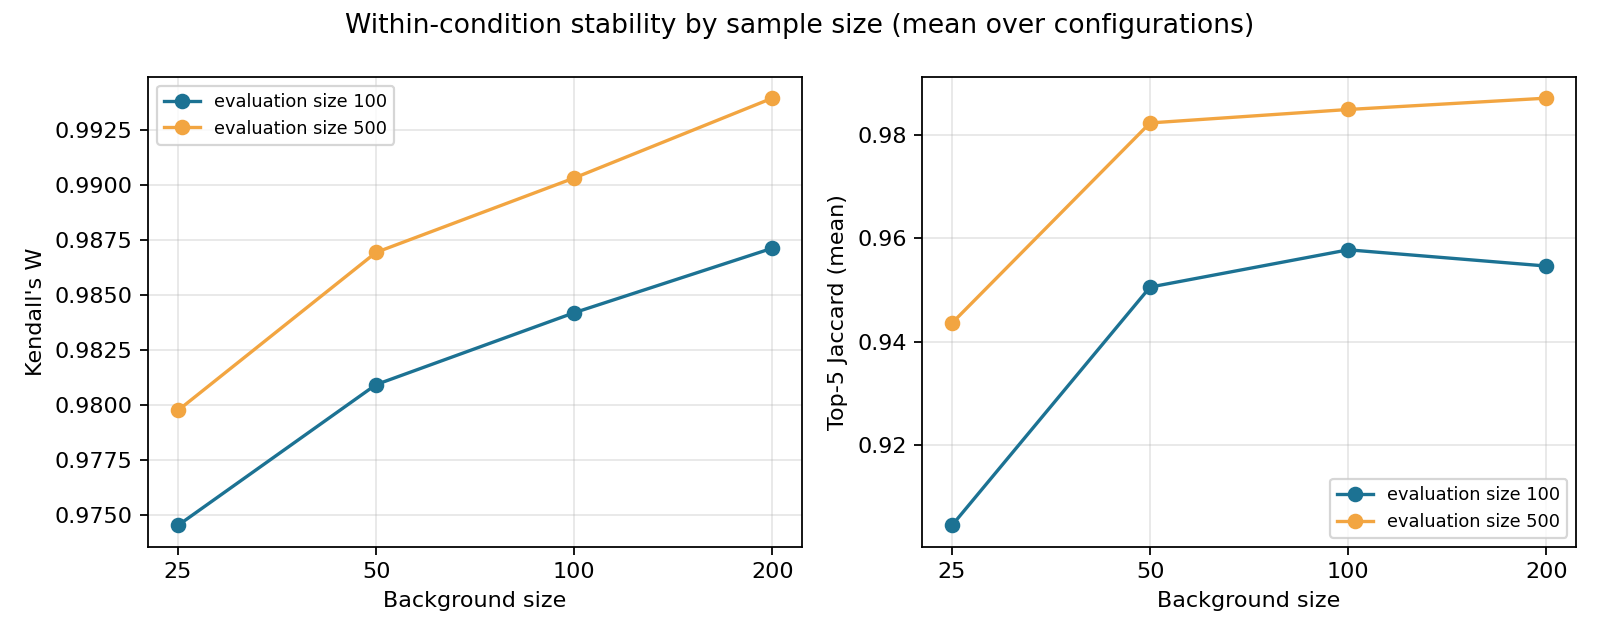
\includegraphics[width=\linewidth]{stability_vs_background_size.png}
\caption{Kendall's $W$ (left) and mean top-5 Jaccard (right) by background size, for each evaluation size, averaged over configurations.}
\label{fig:size}
\end{figure}

\subsubsection{Stability at the top of the ranking}

Which features made the top five depended mainly on the evaluation method ($H = 47.2$, $p < 0.001$), not on the background method ($p = 0.98$). Rare-event sampling was the outlier: over a quarter of its runs produced a top five different from the reference (Table~\ref{tab:evalmethod}).

\begin{table}[htbp]
\centering\small
\caption{Top-five stability by evaluation method.}
\label{tab:evalmethod}
\begin{tabular}{lccc}
\toprule
Evaluation method & Top-5 Jaccard (mean) & Worst seed pair & Runs with a different top 5 \\
\midrule
Uniform & 0.992 & 0.667 & 9 of 720 (1.2\%) \\
Season-stratified & 0.991 & 0.667 & 10 of 720 (1.4\%) \\
Time-stratified & 0.988 & 0.667 & 13 of 720 (1.8\%) \\
Outcome-demand-stratified & 0.943 & 0.429 & 72 of 720 (10.0\%) \\
Rare-event-stratified & 0.876 & 0.429 & 199 of 720 (27.6\%) \\
\bottomrule
\end{tabular}
\end{table}

Post-hoc tests placed rare-event sampling apart from uniform, time- and season-stratified evaluation ($p < 0.001$), while those three were indistinguishable from each other ($p = 1.0$). Season-stratified sampling behaving like uniform is expected: the test split covers only spring and early summer, leaving little seasonal imbalance to correct.

\begin{table}[htbp]
\centering\small
\caption{Mean top-5 Jaccard by evaluation method and evaluation size.}
\label{tab:evalsize}
\begin{tabular}{lcc}
\toprule
Evaluation method & Evaluation 100 & Evaluation 500 \\
\midrule
Uniform & 0.989 & 0.995 \\
Season-stratified & 0.986 & 0.996 \\
Time-stratified & 0.982 & 0.995 \\
Outcome-demand-stratified & 0.894 & 0.993 \\
Rare-event-stratified & 0.858 & 0.894 \\
\bottomrule
\end{tabular}
\end{table}

The last two rows of Table~\ref{tab:evalsize} suggest different causes. Outcome-demand instability behaves like small-sample noise, since five times more evaluation rows almost removes it. Rare-event instability barely responds to more rows, or to larger backgrounds (Figure~\ref{fig:top5}: 0.797 at a 25-row background, 0.912 at 200), which points to a genuine near-tie among the top features under those conditions.

\begin{figure}[htbp]
\centering
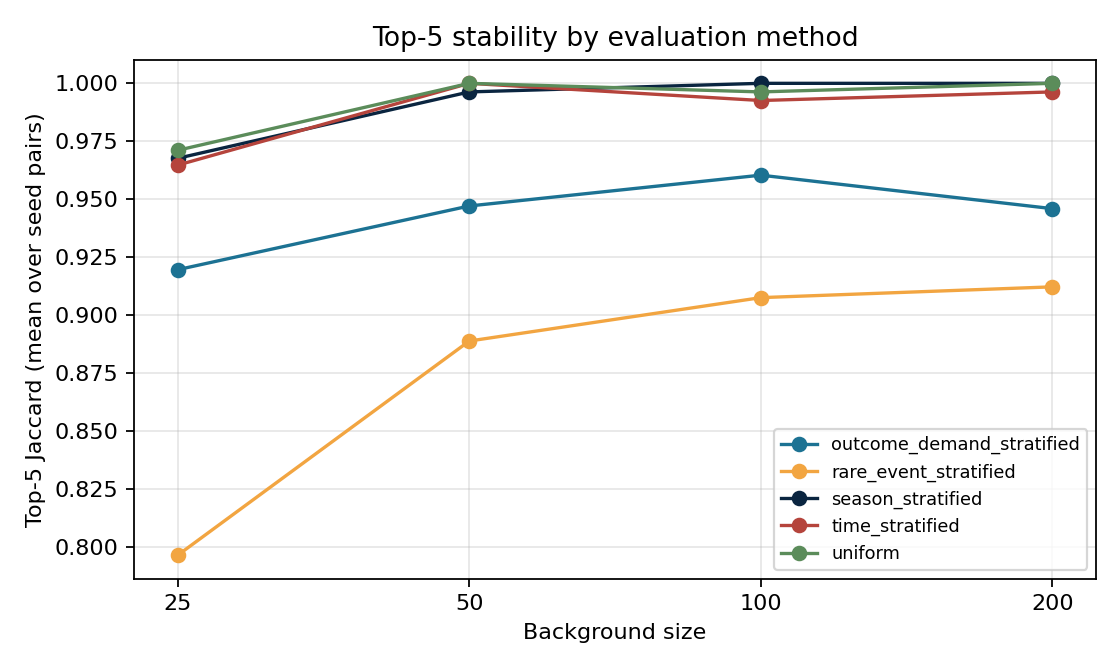
\includegraphics[width=0.8\linewidth]{top5_by_evaluation_method.png}
\caption{Mean top-5 Jaccard by background size for each evaluation method. Rare-event evaluation remains well below the others at every background size.}
\label{fig:top5}
\end{figure}

\subsubsection{Which features change: temperature}

The top-five changes were driven by temperature. When the evaluation sample concentrated on public holidays and extreme-temperature days, maximum temperature gained about a third in importance and rose from eighth to sixth place (Table~\ref{tab:temp}).

\begin{table}[htbp]
\centering\small
\caption{Temperature importance by evaluation method (medians over configurations).}
\label{tab:temp}
\begin{tabular}{lccc}
\toprule
Evaluation method & \feat{temp\_max} mean $|\text{SHAP}|$ (MW) & \feat{temp\_max} rank & \feat{temp\_min} rank \\
\midrule
Uniform & 68.9 & 8 & 12 \\
Season-stratified & 69.3 & 8 & 12 \\
Time-stratified & 69.5 & 8 & 12 \\
Outcome-demand-stratified & 77.7 & 7.5 & 11 \\
Rare-event-stratified & 91.5 & 6 & 10 \\
\bottomrule
\end{tabular}
\end{table}

Under rare-event evaluation, \feat{temp\_max} ranked sixth in all 24 configurations, directly behind the reference top five (\feat{lag\_5min}, \feat{day\_of\_week}, \feat{day\_of\_year}, \feat{origin\_hour\_of\_day}, \feat{lag\_10min}). In 186 of the 199 rare-event runs whose top five differed from the reference, \feat{temp\_max} was the feature that entered, most often displacing \feat{origin\_hour\_of\_day} (121 runs) or \feat{lag\_10min} (65 runs).

Table~\ref{tab:swaps} shows which features entered and left the top five under every evaluation method. Under uniform, time- and season-stratified evaluation, the rare changes were almost always the same swap: \feat{temp\_max} in, \feat{lag\_10min} out. Rare-event evaluation made the same kind of substitution about fifteen times as often, and pushed out \feat{origin\_hour\_of\_day} more often than \feat{lag\_10min}. \feat{temp\_max} is therefore the feature waiting just outside the top five, and explaining extreme conditions is what moves it in. Outcome-demand evaluation behaved differently: there the weekly demand lag, \feat{lag\_1week}, entered in place of a calendar feature, consistent with high-demand periods being driven more by recent weekly patterns than by temperature alone.

\begin{table}[htbp]
\centering\small
\caption{Features entering and leaving the reference top five, in single runs whose top five differed from the reference (720 runs per evaluation method). Counts can exceed the number of changed runs when two features swap at once.}
\label{tab:swaps}
\begin{tabularx}{\linewidth}{l r L L}
\toprule
Evaluation method & Runs changed & Entered (runs) & Left (runs) \\
\midrule
Uniform & 9 & \feat{temp\_max} (9) & \feat{lag\_10min} (8), \feat{origin\_hour\_of\_day} (1) \\
Time-stratified & 13 & \feat{temp\_max} (12), \feat{roll\_mean\_24h} (1) & \feat{lag\_10min} (11), \feat{origin\_hour\_of\_day} (2) \\
Season-stratified & 10 & \feat{temp\_max} (10) & \feat{lag\_10min} (9), \feat{origin\_hour\_of\_day} (1) \\
Rare-event & 199 & \feat{temp\_max} (186), \feat{roll\_mean\_24h} (13) & \feat{origin\_hour\_of\_day} (121), \feat{lag\_10min} (65), \feat{day\_of\_year} (13) \\
Outcome-demand & 72 & \feat{lag\_1week} (68), \feat{temp\_max} (6) & \feat{day\_of\_year} (55), \feat{day\_of\_week} (19) \\
\bottomrule
\end{tabularx}
\end{table}

This is the pattern that motivated the project: global SHAP rankings can understate features whose importance is concentrated in rare conditions~\cite{vanzyl2024}. Averaged over ordinary periods, temperature appears to be a mid-ranked feature; explained over extremes and holidays, it competes for the top five.

\begin{figure}[htbp]
\centering
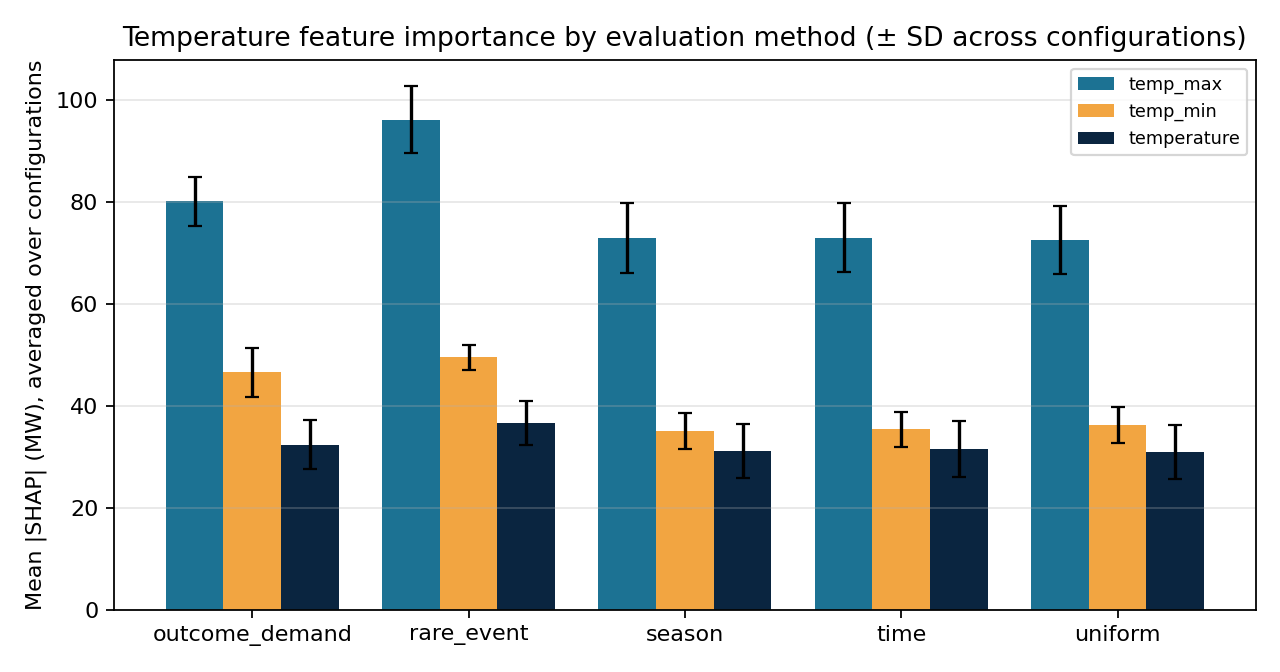
\includegraphics[width=0.8\linewidth]{temperature_importance_by_method.png}
\caption{Mean $|\text{SHAP}|$ of the three temperature features by evaluation method ($\pm$ SD across configurations). Rare-event evaluation raises all three.}
\label{fig:temp}
\end{figure}

Bootstrap confidence intervals over the 30 seeds show how close the contest is (Table~\ref{tab:boot}).

\begin{table}[htbp]
\centering\small
\caption{Mean $|\text{SHAP}|$ (MW) with 95\% bootstrap confidence intervals (2{,}000 resamples of 30 seeds).}
\label{tab:boot}
\begin{tabularx}{\linewidth}{L ccc}
\toprule
Configuration & \feat{origin\_hour\_of\_day} & \feat{temp\_max} & Gap \\
\midrule
Uniform bg 200, uniform eval 500 (reference) & 114.6 [112.9, 116.3] & 65.8 [64.0, 67.6] & 48.8 \\
Uniform bg 200, rare-event eval 500 & 108.5 [107.5, 109.6] & 90.4 [88.4, 92.2] & 18.1 \\
$k$-means bg 200, rare-event eval 500 & 104.5 [103.5, 105.5] & 104.2 [102.9, 105.5] & 0.3 \\
\bottomrule
\end{tabularx}
\end{table}

Under uniform backgrounds the intervals do not overlap, so the consensus order is clear even though individual runs sometimes swap. Under $k$-means with rare-event evaluation the intervals almost coincide: the two features are effectively equal in importance, and averaging more runs would not separate them. Eight of the nine configurations with a fifth-to-sixth gap below 5~MW combine $k$-means backgrounds with rare-event evaluation.

These gaps are comparable to the largest ranking shift the additivity discrepancy can cause (about 1~MW per run, Section~\ref{sec:shap}), so it cannot be excluded as a contributor in those configurations. It does not change the conclusion, since features this close are tied whichever way the order falls; elsewhere the gap exceeds 5~MW and the discrepancy cannot alter the result.

\subsubsection{Does the sampling design change the answer?}

For each configuration, mean $|\text{SHAP}|$ was averaged over its 30 seeds and the features re-ranked, giving a consensus top five that was compared with the reference top five (Section~\ref{sec:metrics}). Every one of the 119 non-reference configurations matched it exactly (Jaccard 1.0 in all 119 comparisons), including all 24 rare-event configurations, where single runs had disagreed most often. The single-run instability above therefore largely disappears when several runs are averaged, although in the near-tied $k$-means and rare-event configurations it does so only narrowly.

Differences appeared further down the ranking. In 77 of the 119 configurations the consensus top ten differed from the reference by exactly one feature, always in the same direction: \feat{lag\_1day}, tenth in the reference, dropped out, and a weather feature entered (\feat{irr\_temperature} in 44 configurations, \feat{temp\_min} in 28, \feat{temperature} in 5). This shift occurred in every configuration using rare-event or outcome-demand evaluation, and in 39 of the 40 using $k$-means backgrounds.

$k$-means backgrounds show that repeatable is not the same as consistent with other designs. They produced the most repeatable rankings ($W$ 0.990) yet agreed least with the reference (Spearman 0.980 and top-10 Jaccard 0.823, against 0.991 and 0.925 for uniform backgrounds). A plausible explanation is that $k$-means selects representatives spread across the feature space rather than in proportion to how common each situation is, over-representing unusual weather in the background; this remains to be verified.

Because the reference itself uses uniform sampling, agreement with it naturally favours uniform designs. Whether the $k$-means and rare-event rankings are less accurate, or answer a different question, is examined in RQ2 (Section~\ref{sec:rq2}).

\subsubsection{Statistical tests}

Background factors significantly affected whole-ranking repeatability, and evaluation method significantly affected the top of the ranking; background method had no effect on the top five or top ten (Table~\ref{tab:kw}). Pairwise Dunn tests for the significant effects are reported in the subsections above.

\begin{table}[htbp]
\centering\small
\caption{Kruskal--Wallis tests on configuration-level values (120 configurations), Holm-corrected across all twelve tests.}
\label{tab:kw}
\begin{tabular}{llrl}
\toprule
Factor & Metric & $H$ & $p$ (Holm) \\
\midrule
Background size & Kendall's $W$ & 44.03 & $<0.001$ \\
 & Top-5 Jaccard & 20.91 & $<0.001$ \\
 & Top-10 Jaccard & 24.77 & $<0.001$ \\
Background method & Kendall's $W$ & 31.19 & $<0.001$ \\
 & Top-5 Jaccard & 0.04 & 0.98 \\
 & Top-10 Jaccard & 3.58 & 0.33 \\
Evaluation size & Kendall's $W$ & 21.43 & $<0.001$ \\
 & Top-5 Jaccard & 13.77 & 0.001 \\
 & Top-10 Jaccard & 5.37 & 0.078 \\
Evaluation method & Kendall's $W$ & 11.74 & 0.078 \\
 & Top-5 Jaccard & 47.15 & $<0.001$ \\
 & Top-10 Jaccard & 55.97 & $<0.001$ \\
\bottomrule
\end{tabular}
\end{table}

\subsubsection{Answer to RQ1}

Background and evaluation choices affect different parts of the ranking: background size and method shape how repeatable the whole ranking is, while evaluation method shapes which features reach the top.
\begin{enumerate}
  \item \textbf{Whole rankings are highly repeatable under every design tested} (Kendall's $W$ 0.963 to 0.997), improving with background size and with $k$-means backgrounds, though gains above 50 rows are small.
  \item \textbf{Top-five membership is design-dependent.} Rare-event evaluation changed the top five in 27.6\% of runs against about 1--2\% for uniform, time- and season-stratified evaluation, and larger samples did not remove the effect.
  \item \textbf{The changes reflect temperature's importance in rare conditions.} Explaining holidays and temperature extremes raises \feat{temp\_max} from eighth to sixth, where it competes for fifth place.
  \item \textbf{Averaging runs recovers a consistent top five,} except that $k$-means backgrounds with rare-event evaluation leave fifth place a genuine tie that averaging cannot break. Designs emphasising unusual conditions also shifted one weather feature into the top ten.
\end{enumerate}
In short, a single SHAP run is dependable for the overall ranking but not necessarily for its top features, especially when explaining rare conditions.

\subsection{RQ2: reliability of rankings}\label{sec:rq2}

The checks provided partial support for SHAP rankings. They agreed substantially with permutation importance, and removing calendar or temperature features increased error under the fixed retraining procedure. However, reliance of the frozen model and incremental utility after retraining are different quantities. Neither establishes a true feature ordering, and the larger temperature-removal effect on rare days was not statistically established.

\subsubsection{Agreement with permutation importance}
Table~\ref{tab:rq2agreement} summarises the 120 configuration comparisons, 40 per background method. Uniform and time-stratified backgrounds agreed slightly more closely with permutation importance than $k$-means, especially on the top ten. Every comparison shared four of the five top features (top-5 Jaccard $4/6 = 0.667$). The differences between background methods are small and, because configurations share permutation rankings, were not tested formally. They do, however, show that the high repeatability of $k$-means rankings did not translate into closer agreement with permutation importance.

The one top-five feature on which the two methods disagreed depended on the evaluation design. In 96 of the 120 configurations (all uniform, time-, season- and rare-event-stratified evaluations), SHAP placed \feat{day\_of\_year} in its top five where permutation importance placed \feat{temp\_max}. Under outcome-demand evaluation, permutation importance instead included \feat{lag\_1week}, in place of \feat{day\_of\_week} with 100 evaluation rows and \feat{day\_of\_year} with 500.

\begin{table}[htbp]
\centering\small
\caption{Mean agreement between SHAP and permutation importance rankings, by background method.}
\label{tab:rq2agreement}
\begin{tabular}{l r r r r}
\toprule
Background & Spearman & Kendall's $\tau$ & Top-5 Jaccard & Top-10 Jaccard \\
\midrule
Uniform & 0.834 & 0.697 & 0.667 & 0.773 \\
Time-stratified & 0.834 & 0.697 & 0.667 & 0.773 \\
$k$-means & 0.830 & 0.690 & 0.667 & 0.724 \\
\bottomrule
\end{tabular}
\end{table}

\subsubsection{Which feature groups matter}
The frozen model's test MAE is 397.49~MW and RMSE 554.50~MW. Table~\ref{tab:rq2ablation} compares group permutation importance with the ablation results. The two answer different questions: permutation shows how much the trained model relies on a group, while ablation shows how much accuracy is lost when the model is retrained without it.

\begin{table}[htbp]
\centering\small
\caption{Feature-group checks on the full test set (MW). Permutation: mean MAE increase over ten shuffles of the frozen model. Ablation: reduced-model error minus its same-seed full-feature control, averaged over three training seeds. Positive values mean worse forecasts.}
\label{tab:rq2ablation}
\begin{tabular}{l r r r}
\toprule
Group & Permutation $\Delta$MAE & Ablation $\Delta$MAE & Ablation $\Delta$RMSE \\
\midrule
Recent demand & 255.03 & $-0.15$ & 4.32 \\
Calendar & 123.74 & 45.45 & 57.40 \\
Temperature & 51.06 & 44.03 & 76.64 \\
Seasonal demand & 49.96 & 8.13 & 13.70 \\
Irradiance & 39.88 & 0.21 & 1.59 \\
Rolling demand & 7.89 & $-14.73$ & $-13.81$ \\
\bottomrule
\end{tabular}
\end{table}

Removing calendar or temperature features raised both MAE and RMSE under the tested training procedure, and seasonal demand had a smaller positive mean removal cost. Recent demand behaved very differently under the two checks: shuffling it caused the largest MAE increase of any group, yet removing it and retraining changed mean MAE by only $-0.15$~MW, although RMSE rose by 4.32~MW. This is consistent with substitution by other demand features, rather than proof that recent demand is unnecessary. Irradiance showed a similar contrast on a smaller scale. Removing rolling-demand features improved the mean errors in these fits. Correlated features, training randomness and the fixed feature-subsampling procedure limit a general feature-removal recommendation.

\subsubsection{Temperature removal on rare and ordinary dates}
Removing the four temperature features increased MAE by 159.11~MW on rare-event days and 35.97~MW on ordinary days, a difference of 123.14~MW. This is the same direction as the RQ1 finding that temperature matters more in rare conditions. However, every bootstrap interval includes zero (Table~\ref{tab:rq2rare}), so with only seven rare-event dates the difference cannot be confirmed. The intervals are also wide, spanning from about $-70$ to $+370$~MW, so the data are consistent both with no rare-day difference and with a much larger one. This result is therefore reported as consistent with the RQ1 finding, not as evidence for it.

\begin{table}[htbp]
\centering\small
\caption{Rare-minus-ordinary paired MAE change after temperature-group removal (MW). Each 95\% origin-date bootstrap interval is conditional on one fitted model pair and uses 1{,}998 valid draws from 2{,}000 attempted draws.}
\label{tab:rq2rare}
\begin{tabular}{r r r r}
\toprule
Training seed & Difference & Lower bound & Upper bound \\
\midrule
2082 & 121.93 & $-71.44$ & 368.11 \\
2083 & 129.90 & $-51.23$ & 355.05 \\
2084 & 117.58 & $-67.23$ & 339.48 \\
\bottomrule
\end{tabular}
\end{table}

Removing \feat{temp\_max} alone increased MAE by 9.50~MW and RMSE by 11.91~MW, with similar point costs on rare and ordinary days (9.78 and 9.48~MW). The larger rare-day point contrast appeared under joint removal of all temperature features, not under this single-feature removal. The checks cannot identify which temperature variable uniquely supplies that information. Permutation results also depended on where the shuffled values came from: shuffling temperature across the whole test set raised rare/ordinary MAE by 90.11/48.32~MW, against 128.34/46.62~MW when values were shuffled only within the same cohort. Permutation importance therefore depends on how the shuffling is done, and should be reported with that design rather than treated as a single true value.

\subsubsection{Answer to RQ2}
\begin{enumerate}
  \item \textbf{SHAP rankings agree substantially, but not fully, with permutation importance} (mean Spearman about 0.83, four of the top five shared). No background method was clearly more faithful than another.
  \item \textbf{Calendar and temperature removal increased error in the tested retraining procedure.} Reliance of the frozen model need not imply the same incremental utility after retraining, especially with correlated demand features.
  \item \textbf{Temperature's larger removal cost on rare days is suggested but not confirmed.} All three conditional contrast intervals include zero. The point contrast appeared for the temperature group, not for \feat{temp\_max} alone.
  \item \textbf{The reliability of the smallest configurations was not tested directly.} The ablations removed feature groups, not each configuration's own top five, so they do not by themselves confirm an RQ3 minimum sample size.
\end{enumerate}

\subsection{RQ3: the smallest sufficient configuration}\label{sec:rq3}

Using the definition of sufficiency in Section~\ref{sec:metrics}, a 50-row background with a 500-row evaluation sample is sufficient for the top five under general evaluation, at about a quarter of the cost of the largest configuration (a 200-row background with a 500-row evaluation sample). The top ten needs 100 rows. Rare-event evaluation is the exception: its top-five stability kept improving up to the largest size tested, so no size within the tested range meets the definition, and 100 rows is recommended as a practical compromise.

\subsubsection{Paired comparisons with the largest size}

Table~\ref{tab:paired} gives median differences from the larger size, with Holm-adjusted Wilcoxon signed-rank $p$-values (Section~\ref{sec:metrics}).

\begin{table}[htbp]
\centering\small
\caption{Paired comparisons with the largest size: median difference ($p$, Holm).}
\label{tab:paired}
\begin{tabular}{lccc}
\toprule
Comparison & Top-5 Jaccard & Top-10 Jaccard & Kendall's $W$ \\
\midrule
Background 25 vs 200 & $-0.043$ ($<0.001$) & $-0.035$ ($<0.001$) & $-0.012$ ($<0.001$) \\
Background 50 vs 200 & $0.000$ (0.77) & $-0.017$ ($<0.001$) & $-0.007$ ($<0.001$) \\
Background 100 vs 200 & $0.000$ (0.88) & $-0.011$ (0.33) & $-0.003$ ($<0.001$) \\
Evaluation 100 vs 500 & $-0.022$ ($<0.001$) & $-0.019$ ($<0.001$) & $-0.006$ ($<0.001$) \\
\bottomrule
\end{tabular}
\end{table}

For the top five, backgrounds of 50 and 100 rows showed no detectable loss: the median difference was zero, and only 17--20\% of pairs scored lower than at 200. A non-significant result is not proof of equivalence, but here the effect itself is also negligible. For the top ten, 100 rows were needed.

Whole-ranking agreement ($W$) was lower at every smaller size in every pair, a consistent but small difference of at most 0.012. $W$ rose by about 0.004 per doubling of the background ($R^2 = 0.38$). Top-five stability did not follow a straight line: almost all of its gain came between 25 and 50 rows, then levelled off (Figure~\ref{fig:size}).

Evaluation samples of 100 were worse than 500 on every metric. Sizes above 500 were not tested, so whether 500 is itself sufficient remains open.

\subsubsection{General and rare-event evaluation}

Pooled results hide one exception. Table~\ref{tab:sufficiency} separates general from rare-event evaluation, with 500 evaluation rows. Under general evaluation (uniform, time-, season- and outcome-demand-stratified), a 50-row background already gave a perfectly stable top five (mean Jaccard 1.000), so doubling it gained nothing; the top ten gained 0.022 from 50 to 100 rows but only 0.008 from 100 to 200, so 100 rows meets the definition there. Under rare-event evaluation, top-five stability rose from 0.805 at 25 rows to 0.912 at 50, 0.925 at 100 and 0.936 at 200. Each doubling beyond 50 rows still added just over 0.01 (0.013, then 0.011), so by the definition used here rare-event stability had not levelled off within the tested range. Even at 200 rows, rare-event top fives remained less stable than general ones at 50. With only six matched pairs per size, these comparisons are descriptive rather than tested.

\begin{table}[htbp]
\centering\small
\caption{Mean top-5 and top-10 Jaccard and SHAP seconds per run by background size, with 500 evaluation rows, for general and rare-event evaluation.}
\label{tab:sufficiency}
\begin{tabular}{r r r r r r r}
\toprule
 & \multicolumn{3}{c}{General evaluation} & \multicolumn{3}{c}{Rare-event evaluation} \\
Background & Top-5 & Top-10 & Seconds & Top-5 & Top-10 & Seconds \\
\midrule
25 & 0.978 & 0.885 & 6.2 & 0.805 & 0.904 & 5.8 \\
50 & 1.000 & 0.913 & 8.9 & 0.912 & 0.928 & 8.3 \\
100 & 1.000 & 0.935 & 16.9 & 0.925 & 0.928 & 18.3 \\
200 & 1.000 & 0.943 & 32.8 & 0.936 & 0.960 & 35.2 \\
\bottomrule
\end{tabular}
\end{table}

\subsubsection{Cost against stability}

SHAP computation time grew steeply with both sizes. A 50-row background with 500 evaluation rows took 8.8 seconds per run against 33.3 seconds for the largest configuration (26\% of the cost), with top-5 Jaccard of 0.982 against 0.987. A 100-row background took 17.2 seconds (52\%). Times cover SHAP computation only, not sample construction (Figure~\ref{fig:cost}).

\begin{figure}[htbp]
\centering
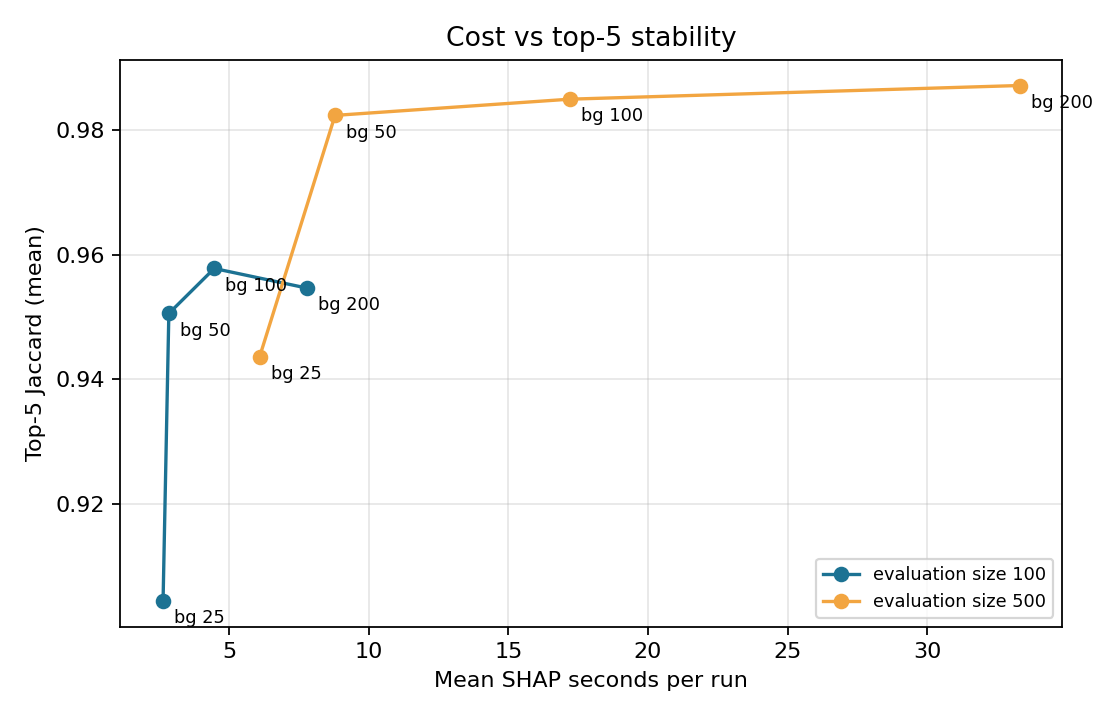
\includegraphics[width=0.75\linewidth]{cost_vs_stability.png}
\caption{Mean SHAP seconds per run against mean top-5 Jaccard for each background size, by evaluation size. Gains flatten beyond a 50-row background while cost keeps rising.}
\label{fig:cost}
\end{figure}

\subsubsection{Reliability by sample size}

Table~\ref{tab:rq2-size-agreement} breaks the 120 SHAP--permutation comparisons from RQ2 down by sample size. Each row averages 15 configurations (three background methods and five evaluation methods). As in RQ2, configurations with the same evaluation method and size share one permutation ranking, so these are descriptive averages rather than independent tests.

\begin{table}[htbp]
\centering\small
\caption{Mean agreement between SHAP and permutation importance rankings by sample size. Each row averages 15 configurations.}
\label{tab:rq2-size-agreement}
\begin{tabular}{r r r r}
\toprule
Background size & Evaluation size & Spearman & Top-10 Jaccard \\
\midrule
25 & 100 & 0.819 & 0.748 \\
25 & 500 & 0.851 & 0.758 \\
50 & 100 & 0.814 & 0.758 \\
50 & 500 & 0.846 & 0.758 \\
100 & 100 & 0.817 & 0.758 \\
100 & 500 & 0.848 & 0.758 \\
200 & 100 & 0.818 & 0.758 \\
200 & 500 & 0.848 & 0.758 \\
\bottomrule
\end{tabular}
\end{table}

Background size made little descriptive difference to agreement with permutation importance: averaged over evaluation sizes, Spearman was 0.835, 0.830, 0.832 and 0.833 for backgrounds of 25, 50, 100 and 200 rows, with no consistent upward trend. Moving from 100 to 500 evaluation rows raised mean Spearman from 0.817 to 0.848. With 500 evaluation rows, the means were 0.8461, 0.8480 and 0.8481 for backgrounds of 50, 100 and 200 rows, respectively; top-10 Jaccard was 0.7576 for all three. These are similar descriptive averages, not evidence of statistical equivalence or proof that larger backgrounds add no reliability benefit.

\subsubsection{Answer to RQ3}

RQ3 asks for the smallest configuration that is both stable and reliable. The descriptive reliability checks showed similar agreement with permutation importance across background sizes and small differences between background methods (Section~\ref{sec:rq2}); they do not establish equivalent reliability or a minimum reliable size. The following recommendations are driven primarily by the stability--cost comparison, with permutation agreement as supporting evidence. A 500-row evaluation sample improved the pooled stability and agreement averages within the tested grid. Table~\ref{tab:recommend} summarises the recommendations.

\begin{table}[htbp]
\centering\small
\caption{Recommended configurations, with 500 evaluation rows throughout. Cost is SHAP time relative to the largest configuration.}
\label{tab:recommend}
\begin{tabularx}{\linewidth}{>{\raggedright\arraybackslash}p{3.6cm} >{\raggedright\arraybackslash}p{3.4cm} r L}
\toprule
Purpose & Background & Cost & Basis \\
\midrule
General evaluation, top five & 50 rows & 26\% & Meets the sufficiency definition: top-five Jaccard 1.000, no gain from larger backgrounds \\
General evaluation, top ten & 100 rows & 52\% & Meets the definition: gain from 100 to 200 rows only 0.008 \\
Rare-event evaluation & 100 rows, averaged over several seeds & 52\% & No size meets the definition; 100 rows reaches 0.925 against 0.936 at 200, at half the cost. Averaging seeds recovered the reference top five in every rare-event configuration \\
Whole-ranking agreement & Largest affordable & -- & Improves slightly at every size tested, with no levelling off \\
\bottomrule
\end{tabularx}
\end{table}

For rare-event analysis, averaging several runs is a more effective remedy than a larger background: even 200 rows left single-run rare-event top fives less stable than general ones at 50, whereas averaging over seeds recovered the reference top five in all 24 rare-event configurations (Section~\ref{sec:rq1}).
One qualification remains. The planned check that removes each configuration's own top five against its bottom five was not carried out (Section~\ref{sec:reliability}), so the reliability side rests on permutation agreement and is weaker than the stability side.

% ===========================================================================
\section{Discussion}\label{sec:discussion}

\subsection{Implications}

\paragraph{Different choices control different parts of the ranking.} Background size and method governed how repeatable the whole ranking was, while evaluation method governed which features reached the top (Table~\ref{tab:kw}). Prior work has focused mainly on background size~\cite{yuan2023}. These results suggest that, for the question practitioners usually ask, ``which features matter most?'', the choice of predictions to explain matters at least as much.

\paragraph{A global ranking answers a narrower question than it appears to.} The same model, explained over ordinary periods and over rare conditions, gave temperature a different importance and a different rank. A ``global'' ranking is therefore global only relative to its evaluation sample: it describes which features matter for the predictions that were explained, consistent with the theoretical result that aggregate SHAP values depend on the distribution they are averaged over~\cite{bhattacharjee2025}. Where decisions concern extreme conditions, such as peak-demand planning, reporting rankings separately for ordinary and rare conditions would be more informative than one pooled ranking.

\paragraph{Whole-ranking metrics can hide the instability that matters most.} Kendall's $W$ never fell below 0.963, a value that would usually be read as excellent agreement, yet some designs changed the top five in over a quarter of runs. This happens because whole-ranking metrics are dominated by the many lower-ranked features, whose order rarely changes. Studies that report only rank correlation risk overstating how dependable the top of a SHAP ranking is.

\paragraph{Repeatable is not the same as right.} $k$-means backgrounds produced the most repeatable rankings yet disagreed most with other designs (Section~\ref{sec:rq1}). Stability alone cannot show which design is closer to the truth, which is why robustness is a necessary but not sufficient property of an explanation~\cite{alvarezmelis2018} and why RQ2 tests reliability separately.

\paragraph{Averaging several small runs may be a better use of compute than one large run.} Averaging over seeds recovered the reference top five in every configuration, and a 50-row background with 500 evaluation rows costs about a quarter of the largest setting. Three such runs would cost less than one large run (26.4 against 33.3 seconds). Whether their average is as stable was not tested directly, but the results suggest it is a promising strategy, mirroring the finding that averaging SHAP values across independently trained models stabilises rankings~\cite{caraker2026}.

\paragraph{Repeatability, model reliance and incremental utility are distinct.} SHAP agreed with permutation importance on four of the top five features in every configuration, yet the checks differed sharply about recent demand: shuffling it raised MAE by 255~MW, while removing it and retraining left mean MAE almost unchanged (Table~\ref{tab:rq2ablation}). This is consistent with substitution by correlated demand features. SHAP attributes model predictions relative to its background, permutation importance measures the frozen model's sensitivity to a specified perturbation, and ablation measures removal cost under a specified retraining procedure. Their agreement is useful supporting evidence, but neither stability nor agreement establishes a causal or uniquely correct feature ordering~\cite{krishna2022}.

\paragraph{The rare-event temperature contrast remains exploratory.} Removing the temperature group cost about 123~MW more MAE on rare-event days than on ordinary days, directionally consistent with the SHAP shift in RQ1. With only seven rare-event dates, however, all three conditional bootstrap intervals include zero. Removing \feat{temp\_max} alone had similar rare and ordinary point costs, which is compatible with substitution by other temperature features but does not identify the mechanism. Under every evaluation design except outcome-demand, permutation importance placed \feat{temp\_max} in the top five where SHAP placed \feat{day\_of\_year}. Rare-event evaluation raised \feat{temp\_max} to sixth in the SHAP ranking, moving it towards the permutation ranking on this feature. The two methods measure different quantities, so this shift does not establish either ranking as correct or demonstrate a larger rare-day removal cost. A new test period with more rare-event dates is needed to test that contrast.

\paragraph{Repeatability did not buy reliability.} $k$-means backgrounds were the most repeatable but agreed slightly less with permutation importance than uniform or time-stratified backgrounds. The difference was small and not tested formally, but it supports the earlier point: a design that gives the same answer every time is not thereby closer to the model's actual behaviour.

\subsection{Relation to prior work}

The results confirm and extend earlier findings. Like Hao et al.~\cite{hao2026}, this study found whole rankings highly consistent in load forecasting, but separating the top five from the rest shows that consistency of the full order can coexist with instability at the top. As Yuan et al.\ found~\cite{yuan2023}, stability improved with background size. Here, however, top-five stability levelled off at about 50 rows. One plausible reason is that exact TreeSHAP removes the explanation-algorithm noise present when Shapley values are approximated, so the remaining variation comes from sampling alone; this was not tested directly. Yuan et al.\ also found the most and least important variables ranked more reliably than the middle; here the instability concentrated at the boundary between fifth and sixth place, consistent with their observation that ranks are least reliable where importances are close.

Liu et al.\ showed that the composition of explanation data affects SHAP output in clinical prediction~\cite{liu2022}, and Laberge et al.\ showed that a deliberately biased background can conceal a feature's importance~\cite{laberge2023}. The rare-event results show that ordinary, well-motivated design choices also shift rankings, without any adversarial intent, and identify which feature responds in electricity demand forecasting: temperature.

Van Zyl et al.\ found that SHAP could underestimate infrequent but important features~\cite{vanzyl2024}. Under ordinary evaluation samples, temperature appeared mid-ranked; focusing on holidays and temperature extremes moved it to the edge of the top five. Abubakkar et al.\ reported the same direction of shift for ERCOT, with temperature reaching the top rank during extreme events~\cite{abubakkar2026}. The present study adds controlled repetition: it shows that the shift is systematic across 24 rare-event configurations and 30 seeds each, and that it is the dominant source of top-five instability. RQ2 adds a further check: removing temperature features cost more on rare days, in the same direction as the SHAP shift, although with too few rare days to confirm it.

\subsection{Limitations}\label{sec:limitations}

\begin{itemize}
  \item \textbf{Seasonal coverage.} Evaluation samples came from a test period of 14 September to 29 December 2025, so the results describe spring and early-summer predictions only. Winter, when heating drives demand, is absent, and the temperature findings may differ there. It also left season-stratified sampling with only two seasons to balance.
  \item \textbf{Weather resolution.} Daily temperature and hourly irradiance were repeated across five-minute rows. The model cannot see temperature changes within a day, which may understate temperature's importance overall, and the repeated values caused the additivity ties described in Section~\ref{sec:shap}. Daily values also introduce a small look-ahead: an origin early in the day sees that day's maximum temperature before it occurs. This may inflate the measured importance of the daily temperature features. It does not affect the stability comparisons, since every configuration explains the same model, but it should be kept in mind when interpreting temperature's importance.
  \item \textbf{Sample-size ranges.} Backgrounds were limited to 200 rows and evaluation samples to 500, so ``the largest available samples'' in RQ3 is a stand-in. Whole-ranking stability was still improving at 200 rows.
  \item \textbf{The reference configuration.} Between-condition agreement was measured against a uniform reference, which naturally favours uniform designs.
  \item \textbf{One trained model.} Rankings were compared for a single frozen model. Retraining with different seeds is a separate source of instability~\cite{caraker2026} that this design deliberately excludes.
  \item \textbf{Scope.} One model type, one region (Victoria), one horizon (24 hours) and one two-year period were studied, so generalisation to other settings is untested.
  \item \textbf{The rare-event definition.} Rare events were defined as public holidays and temperatures outside the 5th--95th percentile range. Other reasonable definitions could change the size of the effect.
  \item \textbf{Statistical design.} Each factor was tested separately, pooling over the others. Interactions, such as rare-event evaluation with background size, were examined descriptively rather than formally, and the rare-event subset in RQ3 had only six matched pairs per size.
  \item \textbf{Group rather than rank-selected ablation.} The RQ2 ablations removed feature groups, not each configuration's own top five against its bottom five, so the reliability side of RQ3 rests on permutation agreement alone.
  \item \textbf{Few rare-event dates.} The test period contained only seven rare-event dates, too few to confirm whether removing temperature costs more on those days.
  \item \textbf{Reconstructed samples and fixed training.} Permutation comparisons used evaluation samples regenerated from saved seeds rather than stored row identifiers, and ablation models kept the original hyperparameters and used three training seeds.
  \item \textbf{Unverified explanations.} The proposed reasons for $k$-means behaviour (Section~\ref{sec:rq1}) and for early saturation of top-five stability (above) remain hypotheses.
\end{itemize}

\subsection{Future work}

\begin{itemize}
  \item \textbf{Extend the size ranges} beyond 200 background and 500 evaluation rows to find where whole-ranking stability levels off.
  \item \textbf{Test averaged small runs directly} against single large runs at equal cost, which could become a simple, cheap recommendation for practitioners.
  \item \textbf{Run the rank-selected ablation} for the recommended 50- and 100-row configurations, removing each configuration's top five against its bottom five, to complete the reliability side of RQ3.
  \item \textbf{Cover all seasons,} for example with a test period that includes winter or with rolling forecast origins. This would also provide more rare-event days for the temperature comparison.
  \item \textbf{Store evaluation row identifiers} with each SHAP run, so later checks can use exactly the same samples.
  \item \textbf{Use higher-resolution weather data} to capture temperature changes within a day and avoid the repeated values that cause additivity ties.
  \item \textbf{Check $k$-means behaviour} by comparing the feature distributions of $k$-means and uniform backgrounds.
  \item \textbf{Model interactions formally,} for example with an aligned-rank-transform analysis of variance.
  \item \textbf{Repeat the study for other regions, horizons and model types} to test how far the findings generalise.
\end{itemize}


% ===========================================================================
\section{Conclusion}\label{sec:conclusion}

This project examined how the choice of background and evaluation samples affects the stability and reliability of global SHAP feature rankings in short-term electricity demand forecasting, using 3{,}600 exact TreeSHAP runs on a frozen LightGBM model of Victorian demand.

For RQ1, whole rankings were highly repeatable under every design, but the top five depended on which predictions were explained: rare-event evaluation changed the top five in over a quarter of runs by raising daily maximum temperature towards fifth place, a shift that averaging over seeds largely resolved. For RQ2, SHAP rankings agreed substantially but not completely with permutation importance, and removing calendar or temperature features increased error under the fixed retraining procedure. Temperature's larger removal cost on rare days was suggestive but not established with the seven rare dates available. For RQ3, a 50-row background with 500 evaluation rows matched the largest configuration's top-five stability at about a quarter of the cost, with 100 rows needed for the top ten; rare-event explanations had no clear sufficient size within the range tested, so 100 rows averaged over several seeds is recommended there. Similar descriptive permutation agreement supports these stability-led recommendations, but does not establish equivalent reliability between designs. The configuration-specific rank-selected ablation remains to be run.

The main practical recommendation is to treat a SHAP ranking as a property of its sampling design: report the background and evaluation samples used, average a few modest-sized runs rather than relying on one, check the top features as well as the whole-ranking correlation, and report rare conditions separately when decisions depend on them.

% ===========================================================================
\bibliographystyle{ieeetr}
\bibliography{refs}


\end{document}
